\documentclass{article}

\usepackage{graphicx}
\usepackage{hyperref}

\title{User Interface Parsing \\ \small{Progress Update}}
\author{Calvin Loncaric}
\date{April 29, 2015}

\begin{document}

\maketitle

\noindent Since the last update I have been working on stroke cleanup and
classification. See \autoref{fig:screenshot} for an example on a very simple
layout. Since the last update I:
\begin{itemize}
\item improved line grouping algorithm,
\item began tuning the Tesseract OCR software,
\item implemented a ``voting'' system where each line votes for a likely
    explanation for itself \emph{and} its neighbors.
\end{itemize}

\noindent My immediate next steps are:
\begin{itemize}
\item start implementing high-level element recognition (i.e. find the boxes).
\end{itemize}

\begin{figure}
    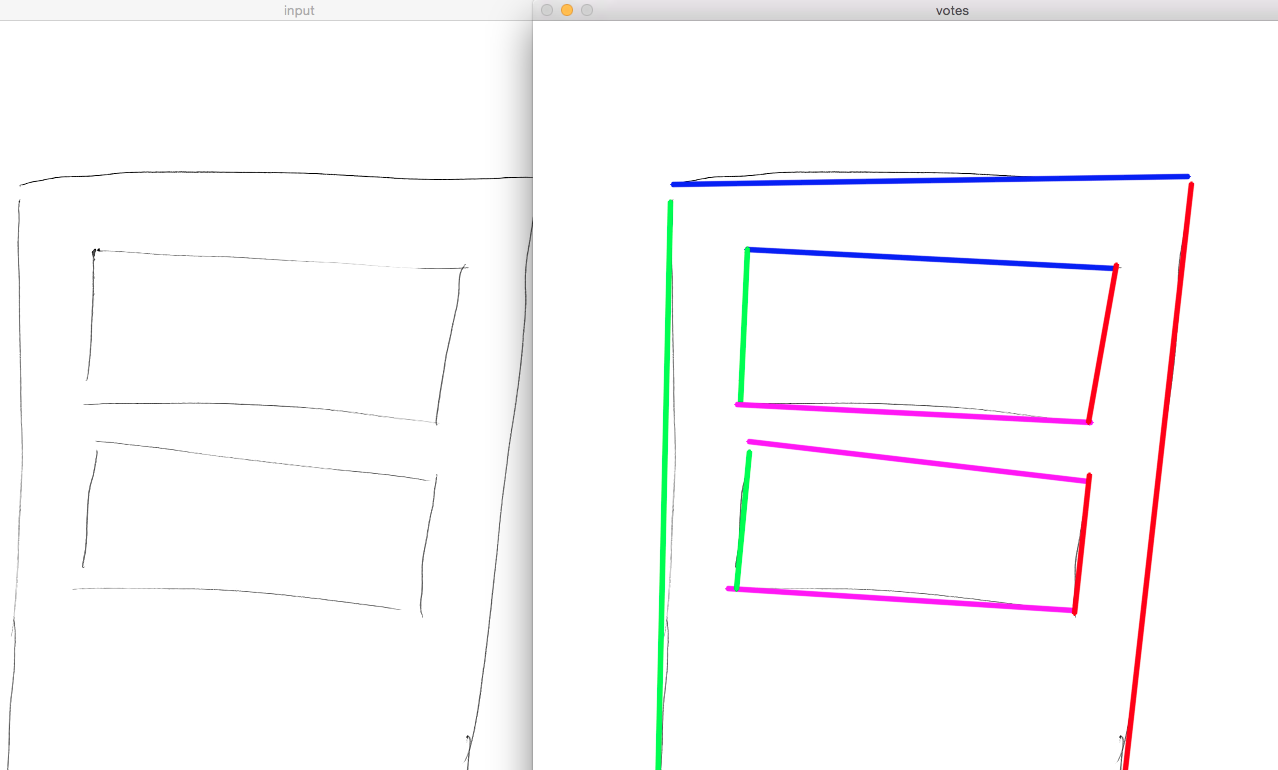
\includegraphics[width=\textwidth]{progress-2015-04-29-screenshot.png}
    \caption{Stroke cleanup and classification (top, right, left, or bottom
        edge). The one misclassified line actually has an equal number of votes
        for the correct classification; it will be properly handled by the next
        step (unimplemented).}
    \label{fig:screenshot}
\end{figure}

\end{document}
